\newthought{Select exercises on sequences and series} from Chapter 3 of the \textit{Lectures on Real Analysis} textbook\footnote{\bibentry{lárusson2012lectures}}.

\begin{tcolorbox}[title={Exercise 3.17, page 35}]
(a) Let $a \geq 0$ and $n \in \mathbb{N}$, $n \geq 2$. Show that 

$$
(1 + a)^n \geq \frac{1}{2} n (n -1)a^2
$$

(b) Show that $n^{\frac{1}{n}} \to 1$ as $n \to \infty$.
\end{tcolorbox}

\begin{solution}
(a) Using the binomial expansion, we get

$$
(1 + a)^n = \sum_{k = 0}^n \binom{n}{k} a^k = 1 + n a + \frac{1}{2} n (n -1)a^2 + \ldots \geq \frac{1}{2} n (n -1)a^2
$$

(b) Using the inequality from (a) with $a = n^{\frac{1}{n}} - 1$ we get

$$
n = (n^{\frac{1}{n}} - 1 + 1)^n \geq \frac{1}{2} n (n -1) (n^{\frac{1}{n}} - 1)
$$

So $\frac{2}{n-1} \geq (n^{\frac{1}{n}} - 1)$ and $n^{\frac{1}{n}} \to 1$.
\end{solution}

\begin{tcolorbox}[title={Exercise 3.18, page 35}]
Consider the recursively defined sequence $(a_n)$ with $a_1 = 3$ and $a_{n+1}=\frac{a_n}{2} + \frac{3}{a_n}$. Show that $(a_n)$ converges and find its limit.
\end{tcolorbox}

\begin{solution}
Let's first prove by induction that $\forall n \in \mathbb{N}: 2 < a_n \leq 3$:

It's true for $a_1=3$. Assume it is true for a given $n$ and let's do the induction step.

$$
a_{n+1} = \frac{a_n}{2} + \frac{3}{a_n} > \frac{2}{2} + \frac{3}{3} = 2
$$

Also

$$
a_{n+1} = \frac{a_n}{2} + \frac{3}{a_n} \leq \frac{3}{2} + \frac{3}{2} = 3
$$

At least we know $(a_n)$ is bounded. Let us spy a little and assume $(a_n)$ does converge, say to limit $L$. Then $L$ must satisfy: 

$$
L = \frac{L}{2} + \frac{3}{L}
$$

which works out to $L = \sqrt{6}$.

Let's try with a simpler sequence $(b_n)$ such that $a_n = b_n \sqrt{6}$. 

\begin{align*}
  a_{n+1} = b_{n + 1} \sqrt{6} &= \frac{a_n}{2} + \frac{3}{a_n} \\
                              &= \frac{b_n \sqrt{6}}{2} + \frac{3}{b_n \sqrt{6}} \\
                              &= \frac{b_n \sqrt{6}}{2} + \frac{\sqrt{6}}{2 b_n}
\end{align*}

So $(b_n)$ satisfies $b_{n+1} = \frac{1}{2}(b_n + \frac{1}{b_n})$. We prove that $(b_n)$ is monoton decreasing:

\begin{align*}
  b_{n+1} \leq b_n & \Leftrightarrow \\
  \frac{1}{2}(b_n + \frac{1}{n}) \leq b_n & \Leftrightarrow \\
  b_n^2 + 1 \leq 2 b_n^2  & \Leftrightarrow \\
  b_n^2 \geq 1 & \Leftrightarrow \\
  b_n \geq 1
\end{align*}

We use the AGM inequality\footnote{For positive $x$ and $y$ we have $(\sqrt{x} + \sqrt{y})^2 \geq 0$ which when expanded ends up at $\frac{x + y}{2} \geq \sqrt{xy}$. } and show:

$$
b_{n+1} = \frac{1}{2}(b_n + \frac{1}{b_n}) \geq \sqrt{b_n \frac{1}{b_n}} = 1
$$

So $(b_n)$ is monoton decreasing and bounded below by $1$, so $(b_n)$ converges, and so does $(a_n)$: $b_n \to 1$ and $a_n \to \sqrt{6}$.

\end{solution}

\begin{tcolorbox}[title={Exercise 3.23, page 36}]
Let $\sum a_n$ be a series. Set $a^+_n = max\{0, a_n\}$ and $a^-_n = min\{0, a_n\}$. Consider the series $\sum a^+_n$ and $\sum a^-_n$.

(a) Prove that $\sum a_n$ is absolutely convergent if and only if $\sum a^+_n$ and $\sum a^-_n$ both converge. Then $\sum a_n = \sum a^+_n + \sum a^-_n$.

(b) Prove that if $\sum a_n$ is conditionally convergent, then $\sum a^+_n$ and $\sum a^-_n$ both diverge. 
\end{tcolorbox}

\begin{solution}
We will use the partial sums:

\begin{align*}
s_n &= \sum_{k = 1}^n a_k, \quad s^a_n = \sum_{k = 1}^n |a_k| \\
s^+_n &= \sum_{k = 1}^n a^+_k, \quad s^-_n = \sum_{k = 1}^n a^-_k
\end{align*}

(a) $(\Rightarrow)$ 

We have $\forall n \in \mathbb{N}: |a_n| \geq a^+_n \text{ and } |a_n| \geq (-1) a^-_n$. Using the comparison test we find $\sum a^+_n$ and $\sum a^-_n$ converge.

$(\Leftarrow)$ $\sum a^+_n$ and $\sum a^-_n$ converge, so then also $\sum a^+_n + (-1) \sum a^-_n$ converges. But $s^a_n = s^+_n + (-1)s^-_n$, so $\sum |a_n|$ converges too.

(b) $\sum a_n$ converges conditionally. If both $\sum a^+_n$ and $\sum a^-_n$ converge, then from (a) we would have $\sum a_n$ converges absolutely, contradicting the premise. So at least one of $\sum a^+_n$ or $\sum a^-_n$ must diverge. 

Assume $\sum a^+_n$ diverges (the other case is similar). $s^+_n$ is monotonically increasing and divergent, so it is unbounded. We have $s^+_n = s_n - s^-_n$ and $s_n$ is bounded. It follows that $s^-_n$ has to be unbounded, so $\sum a^-_n$ diverges also.

\end{solution}

\begin{tcolorbox}[title={Exercise 3.24, page 36}]
Let $\sum a_n$ be a conditionally convergent series. Prove that for every $\sigma \in \mathbb{R}$ there is a rearrangement of $\sum a_n$ that converges to $\sigma$.
\end{tcolorbox}

\begin{solution}
We will construct this rearrangement.

We know from the previous exercise that both $\sum a^+_n$ and $\sum a^-_n$ diverge and both $s^+_n$ and $s^-_n$ are unbounded. 

Assume first that $\sigma > 0$ (the other case is similar). Since $s^+_n$ is unbounded, there exists\footnote{This $N_1$ has to exist because $s^+_n$ is unbounded. If it was only zeros it would converge and be bounded.} a $N_1 \in \mathbb{N}$ such that 

\begin{align*}
\sum_{k = 1}^{N_1-1} a^+_k  &\leq \sigma \\
\sum_{k = 1}^{N_1} a^+_k &> \sigma
\end{align*}

Let $d_1 = |\sum_{k = 1}^{N_1} a^+_k - \sigma|$. We see that $0 < d_1 \leq |a^+_{N_1}|$. Our rearrangement will start with the first $N_1$ terms from $\sum a^+_n$. For the next terms we turn to $\sum a^-_n$. $s^-_n$ is also unbounded, so there exists a $M_1 \in \mathbb{N}$ such that

\begin{align*}
\sum_{k = 1}^{M_1-1} a^-_k &\geq d_1 \\
\sum_{k = 1}^{M_1} a^-_k &< d_1
\end{align*}

We add the first $M_1$ terms from $\sum a^-_n$ to the rearrangement. Let $d_2 = |\sum_{k = 1}^{N_1} a^+_k + \sum_{k = 1}^{M_1} a^-_k - \sigma|$. We see that $0 < d_2 \leq |a^-_{M_1}|$.

Next we go back to $\sum a^+_n$ for more terms. The tail of $\sum a^+_n$ starting at $N_1 + 1$ is also unbounded, so there must exist a $N_2$ such that

\begin{align*}
\sum_{k = N_1 + 1}^{N_2-1} a^+_k  &\leq d_2 \\
\sum_{k = N_1 + 1}^{N_2} a^+_k &> d_2
\end{align*}

We add the terms $\sum_{k = N_1 + 1}^{N_2} a^+_k$ to the rearrangement and define 

$$
d_3 = |\sum_{k = 1}^{N_1} a^+_k + \sum_{k = 1}^{M_1} a^-_k + \sum_{k = N_1 + 1}^{N_2} a^+_k - \sigma|
$$

We see that $0 < d_3 \leq |a^+_{N_2}|$.

We go back down with the help of terms from the tail of $\sum a^-_n$ starting at $M_1$, a tail that is also unbounded. There must exist a $M_2$ such that

\begin{align*}
\sum_{k = M_1 + 1}^{M_2-1} a^+_k  &\geq d_3 \\
\sum_{k = M_1 + 1}^{M_2} a^+_k & < d_3
\end{align*}

We add the terms $\sum_{k = M_1 + 1}^{M_2} a^-_k$ to the rearrangement and define 

$$
d_4 = |\sum_{k = 1}^{N_1} a^+_k + \sum_{k = 1}^{M_1} a^-_k + \sum_{k = N_1 + 1}^{N_2} a^+_k + \sum_{k = M_1 + 1}^{M_2} a^-_k - \sigma|
$$

We see that $0 < d_4 \leq |a^-_{M_2}|$.

We continue in this way, switching between terms in $\sum a^+_n$ and $\sum a^-_n$, constructing a rearrangement of $\sum a_n$ that has partial sums that have distance $d_n$ from $\sigma$.

The sequence $(d_n)$ of distances is bounded by $(|a_n|)$ and $\sum a_n$ is a conditionally convergent series, so $a_n \to 0$. That means that $d_n \to 0$ and the rearrangement converges to $\sigma$.

\end{solution}

\begin{tcolorbox}[title={Exercise 3.30, page 37}]
Show that there is a sequence $(a_n)$ such that for every real number $x$, there is a subsequence of $(a_n)$ converging to $x$.
\end{tcolorbox}

\begin{solution}
At first glance this seems quite a fantastical premise. How can there be a sequence that for every real number contains a subsequence converging to that number? Isn't $\mathbb{R}$ uncountable?
Well, the best way to prove the existence of such a sequence is to construct it.

First we want to make our life easier: we use the fact that there exists a bijection between the interval $(0, 1)$ and $\mathbb{R}$. There are many bijections between these two sets to choose from and we will choose a continuous one:

\begin{align*}
  F: \mathbb{R} &\to (0, 1) \\
  F(x) &= \frac{1}{1 + e^x} 
\end{align*}

and its inverse

\begin{align*}
  F^{-1}: (0, 1) &\to \mathbb{R} \\
  F^{-1}(x) &= \ln(\frac{1 - x}{x}) 
\end{align*}

If we can construct subsequences that converge to $x \in (0, 1)$ then we can use $F^{-1}$ to map them over to $y \in \mathbb{R}$ and because of continuity the mapping of the subsequence will converge to $y$. The construction idea is to map a given $n \in \mathbb{N}$ to a pair $(i, j) \in \mathbb{N} \times \mathbb{N}$. This $(i, j)$ pair will have the following meaning: $j$ subdivides $(0, 1)$ into $j$ subintervals of length $\frac{1}{j}$ and $i$ will select which of those $j$ subintervals we mean. A given $x \in (0, 1)$ will fall into one of them and its corresponding $(i, j)$ pair will determine the $n$ we use in the subsequence. Increasing the $j$ and then choosing the corresponding $i$ subinterval containing $x$ will get us closer and closer to $x$.

This is the construction idea. We still have to deal with the technicalities.

First we want a bijection from $\mathbb{N}$ to a subset of $\mathbb{N} \times \mathbb{N}$ where the pairs $(i, j)$ satisfy $i \leq j$. We use a similar approach to the one we used in a previous note: \url{https://sagenhaft.space/posts/math_notes/counting/counting.pdf}.

\begin{marginfigure}[1.0in]
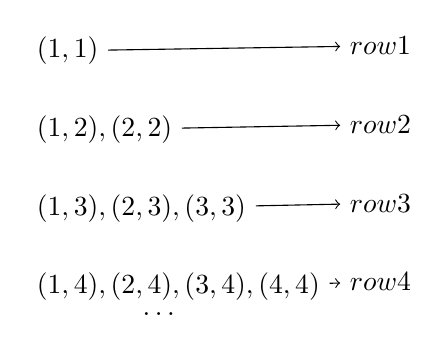
\begin{tikzpicture}
 \node at (-2, 3)  (1l) [anchor=north west] {$(1, 1)$};
 \node at (3, 3)  (1r) [anchor=north east] {$\text{row } 1$};
 \node at (-2, 2)  (2l) [anchor=north west] {$(1, 2), (2, 2)$};
 \node at (3, 2)  (2r) [anchor=north east] {$\text{row } 2$};
 \node at (-2, 1)  (3l) [anchor=north west] {$(1, 3), (2, 3), (3, 3)$};
 \node at (3, 1)  (3r) [anchor=north east] {$\text{row } 3$};
 \node at (-2, 0)  (4l) [anchor=north west] {$(1, 4), (2, 4), (3, 4), (4, 4)$};
 \node at (3, 0)  (4r) [anchor=north east] {$\text{row } 4$};
 \node at (0, -0.5) [anchor=north east] {$\dots$};
 \draw [->] (1l) -- (1r);
 \draw [->] (2l) -- (2r);
 \draw [->] (3l) -- (3r);
 \draw [->] (4l) -- (4r);
\end{tikzpicture}
\caption{Going from $n$ to $(i, j)$ with $i \leq j$.}
\label{fig:counting:series}
\end{marginfigure}

We order the pairs $(i, j) \in \mathbb{N} \times \mathbb{N}$ satisfying $i \leq j$ in rows, such that row $r$ has pairs $(1, r), (2, r), \ldots, (r, r)$. Figure \ref{fig:counting:series} illustrates the idea. Our bijection will count going down the rows and going left to right in each row. So the order is $(1, 1), (1, 2), (2, 2), (1, 3), (2, 3), (3, 3), \ldots$

Lets first deduce the inverse, going from $(i, j)$ to $n$ in that order. For a given $(i, j)$ we know we are in row $j$ at pair $i$ in that row. Each row $k$ before row $j$ has $k$ pairs in it, therefore the corresponding position $n$ in the counting order is: 

\begin{align*}
n &= \sum_{k = 1}^{j - 1} k + i \\
  &=  \frac{j (j - 1)}{2} + i
\end{align*}

We can test this: in the Figure \ref{fig:counting:series}, pair $(2, 4)$ should be the eighth pair. $\frac{4 \times 3}{2} + 2 = 8$, so it checks out. We denote $M = \{ (i, j) \in \mathbb{N} \times \mathbb{N}:i \leq j\}$ and define the function $f$:

\begin{align*}
f: M &\to \mathbb{N} \\
f(i, j) &= \frac{j (j - 1)}{2} + i
\end{align*}

It is easy to prove that $f$ is a bijection. Suppose we have two pairs $(i_1, j_1) \ne (i_2, j_2)$. If $j_1 \ne j_2$ then they are in different rows. If $j_1 = j_2$ then we must have $i_1 \ne i_2$, so again their mapping is different. It follows that $f$ is injective.

Given $n \in \mathbb{N}$, can we find $(i, j)$ such that $f(i, j) = n$? The $n$th pair falls on some row $r$. There are $\frac{r (r - 1)}{2}$ pairs in the rows before row $r$ and $\frac{r (r + 1)}{2}$ pairs in the first $r$ rows. Therefore:

$$
\frac{r (r - 1)}{2} < n \leq \frac{r (r + 1)}{2}
$$

The two relevant values for these two quadratic inequalities are $\frac{1 + \sqrt{1 + 8 n}}{2}$ and $\frac{-1 + \sqrt{1 + 8 n}}{2}$ because we have to stay positive. Notice that their difference is $\frac{1 + \sqrt{1 + 8 n}}{2} - \frac{-1 + \sqrt{1 + 8 n}}{2} = 1$, so there is only one positive integer satisfying both inequalities (as we hoped) and that positive integer is our sought after row $r$:

$$
r = \bigg\lceil \frac{-1 + \sqrt{1 + 8 n}}{2} \bigg\rceil
$$

Lets verify this for fun again, making sure that the eighth pair is on row four: 
$$
\bigg\lceil \frac{-1 + \sqrt{1 + 8 \times 8}}{2} \bigg\rceil = \bigg\lceil \frac{-1 + \sqrt{65}}{2} \bigg\rceil = \lceil 3.53113 \rceil = 4
$$

We know that $j = r$ and then $i = n - \frac{j (j - 1)}{2}$. This means that $f$ is surjective and therefore a bijection.

The inverse $f^{-1}(n)$ is:

\begin{align*}
f^{-1}: \mathbb{N} &\to M \\
f^{-1}(n) &= (i, j) \text{, where } j = \bigg\lceil \frac{-1 + \sqrt{1 + 8 n}}{2} \bigg\rceil \text{ and } i = n - \frac{j (j - 1)}{2}
\end{align*}


For a given pair $(i, j)$ lets divide interval $(0, 1)$ into $j$ non-overlapping intervals: 
$$
(0, \frac{1}{j}], (\frac{1}{j}, \frac{2}{j}], \ldots, (\frac{j - 2}{j}, \frac{j - 1}{j}], (\frac{j-1}{j}, 1)
$$

Except for the last subinterval, all other subintervals are left-exclusive and right-inclusive. The last one is open on both ends. This is just a technicality, but we now have a set of intervals that don't intersect and their union is $(0, 1)$.

A given $x \in (0, 1)$ will fall into one of these subintervals. We will use this fact shortly.

We are ready to define our sequence $(a_n)$:

$$
a_n = \ln(\frac{j - i}{i}) \text{, where } j = \bigg\lceil \frac{-1 + \sqrt{1 + 8 n}}{2} \bigg\rceil \text{ and } i = n - \frac{j (j - 1)}{2}
$$

For any $x \in \mathbb{R}$ we first get $y = F(x) = \frac{1}{1 + e^x}$ which places us in interval $(0, 1)$. We choose the following subsequence of $(a_{n_k})$: choose the $n_k$ so that the corresponding $(i, j)$ pair according to our bijection $f^{-1}$ is the $i$th interval of the division of $(0, 1)$ into $j$ non-overlapping intervals that contains $y$. Keep increasing $j$ and selecting the corresponding $(a_{n_k})$ according to this criteria. This subsequence converges to $x$. 

This construction is not unique. We made pretty arbitrary choices along the way. There are more than one sequence $(a_n)$ with the desired property.

\end{solution}
